% Faculty brief: progress up to Sprint 4. Build: E:\tools\tectonic\tectonic.exe ShelfSense_Brief_Report.tex
\documentclass[10pt,a4paper]{article}
\usepackage[margin=2cm]{geometry}
\usepackage{graphicx}
\usepackage{booktabs}
\usepackage{float}
\usepackage{xcolor}
\usepackage{enumitem}
\usepackage[hidelinks]{hyperref}
\setlist{nosep,leftmargin=*}
\setlength{\parskip}{4pt}
\setlength{\parindent}{0pt}
\graphicspath{{../weekly_reports/figures/}}

\begin{document}

\begin{center}
{\LARGE\bfseries ShelfSense: AI-Based Retail Merchandising Audit}\\[4pt]
{\large Progress brief, Sprints 1--4}\\[6pt]
CSE499A, Section 13, Group 1\\
Syed Ashfaq Shafin, Sadid Mehal Habib, Shafil Ahmed, Rutaba Adiba Rahman\\
North South University, 18 October 2026
\end{center}

\section*{Summary}
ShelfSense turns a merchandiser's phone video of store shelves into an audit report backed by
evidence. Sprints 1--3 are complete. In Sprint 4 we recorded 111 supermarket videos, trained a
product detector that reaches \textbf{mAP50 0.913} on SKU-110K, and showed that asking the
vision-language model (VLM) about one detected product at a time \textbf{doubles the brands it
finds} (recall 0.30 $\rightarrow$ 0.63) compared with asking about the whole frame.

\section*{Problem and approach}
Brand companies (Coca-Cola, Pepsi/Transcom, Akij, \dots) pay shops for branded fridges and prime
shelf placement, and send field auditors to check compliance. Auditors can be bribed and report
false results. ShelfSense replaces the auditor's word with \emph{verifiable evidence}: every finding
points to a keyframe and timestamp a person can check. Because a false ``competitor in your
fridge'' accuses an honest shopkeeper, the system favours \emph{precision over recall} for
violations. Key KPIs: cooler purity, paid placement, out-of-stock and share of shelf.

VLMs cannot count densely packed products, so the pipeline is hybrid:
\textbf{(1)} extract sharp, non-duplicate keyframes $\rightarrow$
\textbf{(2)} a YOLO nano detector finds every product $\rightarrow$
\textbf{(3)} a small VLM (Qwen2-VL-2B) reads the brand of each product crop $\rightarrow$
\textbf{(4)} rules compute the KPIs and write the report.
Everything runs on student hardware: laptops and free Kaggle GPUs.

\section*{Progress by sprint}
\begin{center}
\small
\begin{tabular}{@{}l p{4.2cm} l p{6.6cm}@{}}
\toprule
Sprint & Focus & Status & Main result \\
\midrule
1 & Setup and problem definition & Done & Scope, KPIs, repository, six-sprint plan \\
2 & Data and keyframe extraction & Done & Extractor with blur and duplicate filters; Crete blur score replaced Laplacian variance, which failed on real video \\
3 & Baseline VLM (zero-shot) & Done & Prompts fixed the answer format but not perception: invented brands (precision 0.13--0.30), every count ``10'' \\
4 & Product detection & Mostly done & Detector mAP50 0.913; crop-based brand reading doubles recall; mAP on our own frames pending corrected labels \\
5 & Integration and rule engine & Next & End-to-end JSON audit report \\
6 & Evaluation and demo & Planned & Metrics against manual counts, demo app \\
\bottomrule
\end{tabular}
\end{center}

\section*{Latest update (Sprint 4)}

\subsection*{New footage}
111 own shelf videos from a Bangladeshi supermarket (about 22 minutes; duplicates found by SHA-256
and stock clips removed). Split into 82 train and 29 test videos by blocks of neighbouring clips, so
the same shelf never appears in both sets. Keyframe extraction kept 4{,}491 of 5{,}069 sampled
frames; the videos gave the first real test of the blur filter.

\subsection*{Product detector}
YOLOv8n, one class \emph{product}, trained on 2{,}000 SKU-110K shelf photos (30 epochs, 2.7 hours
on a 4\,GB laptop GPU) and evaluated on 500 held-out photos.
\begin{center}
\small
\begin{tabular}{@{}lcccc@{}}
\toprule
Setting & mAP50 & mAP50-95 & Precision & Recall \\
\midrule
1{,}024\,px, up to 1{,}000 boxes per image (chosen) & \textbf{0.913} & \textbf{0.564} & 0.897 & 0.844 \\
1{,}024\,px, up to 299 boxes & 0.889 & 0.549 & 0.897 & 0.833 \\
640\,px (default), up to 1{,}000 boxes & 0.866 & 0.510 & 0.875 & 0.792 \\
\bottomrule
\end{tabular}
\end{center}
Dense shelves need both settings: one photo holds 718 products. On all 4{,}558 keyframes (our videos
plus 67 from the stock clips) the detector found 151{,}279 products (median 29 per frame). It works on packed shelves seen from a
normal distance but misses large products close to the camera (Fig.~\ref{fig:det}).

\begin{figure}[h]
\centering
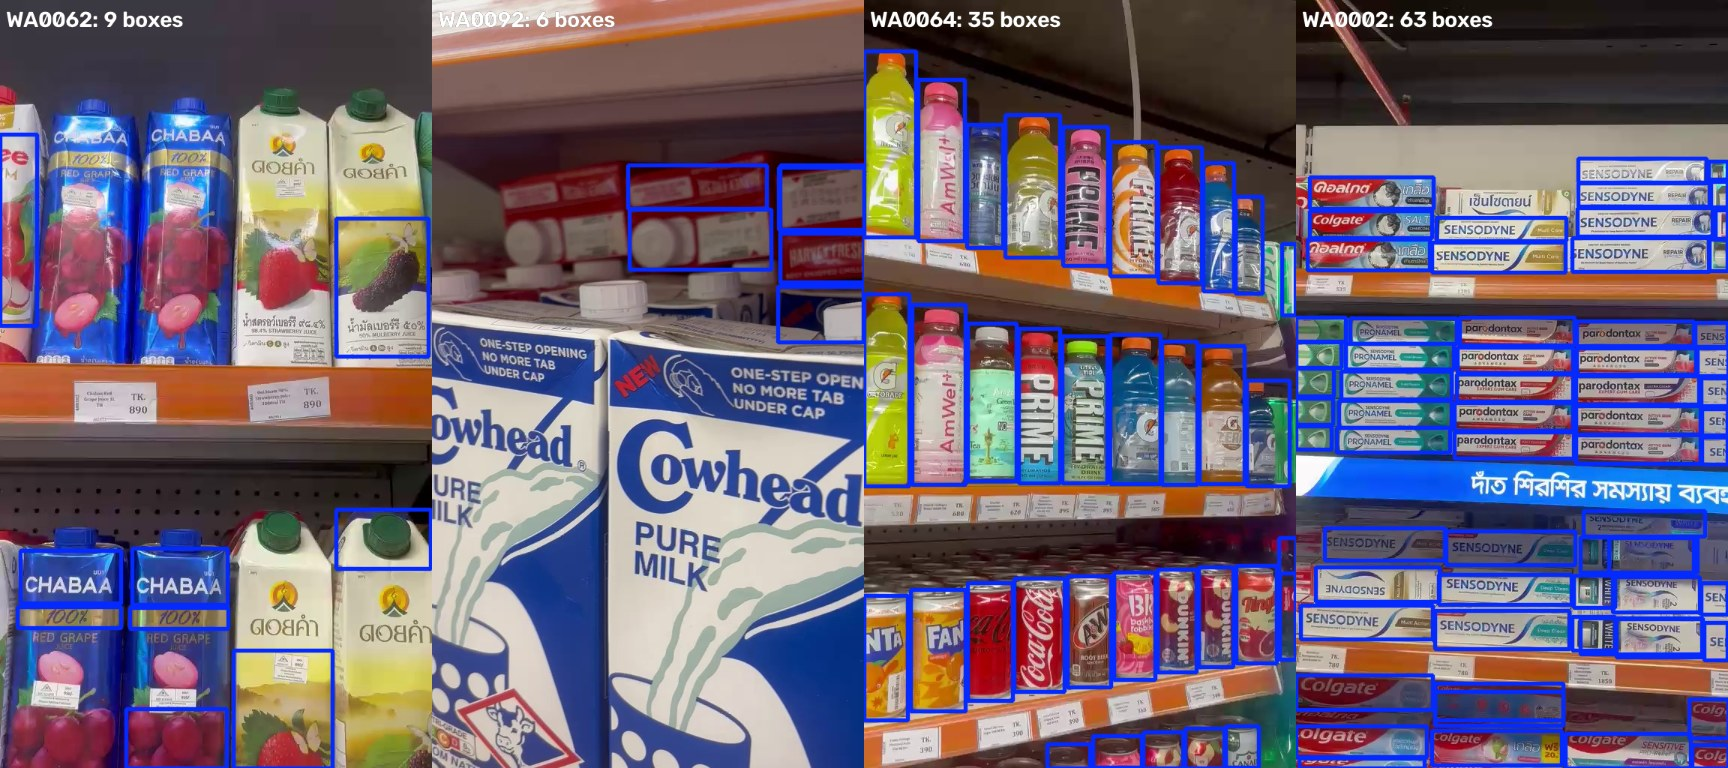
\includegraphics[width=0.72\linewidth]{detector_good_and_bad.jpg}
\caption{Detector on our test videos. Left: large close-up cartons are missed. Right: packed
shelves, where nearly every product is found.}
\label{fig:det}
\end{figure}

\subsection*{Brand reading: product crops vs whole frames}
On 12 frames from six drinks-shelf test videos we asked the same Qwen2-VL-2B model to list the
brands in the whole frame, and to name the brand of 120 single-product crops cut by the detector.
\begin{center}
\small
\begin{tabular}{@{}lccc@{}}
\toprule
Method & Usable answers & Brand precision & Brand recall \\
\midrule
Whole frame, ``list the brands'' & 6 of 12 & 1.00 (6 frames) & 0.30 \\
Detector crops, ``which brand is this?'' & 12 of 12 & 0.94 & \textbf{0.63} \\
\bottomrule
\end{tabular}
\end{center}
Half of the whole-frame answers got stuck repeating words and gave no list. On crops, 48 of 67
readable products were named correctly. Wrong brands were rare (2 of 120) but both were
``Coca-Cola'', so a person must still check the evidence before a violation is reported
(Fig.~\ref{fig:crops}). Brand labels for this test are drafts awaiting a team check; answers were
matched to the list of 24 expected brands, so the numbers are an upper bound.

\begin{figure}[H]
\centering
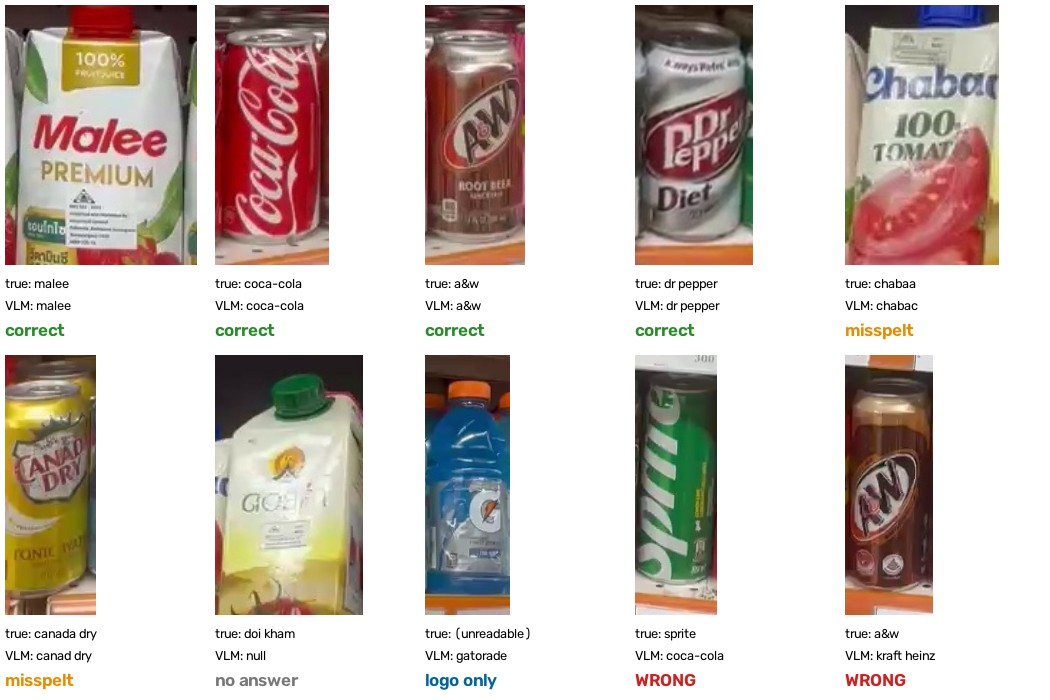
\includegraphics[width=0.8\linewidth]{crop_brand_examples.jpg}
\caption{Single-product crops with the true brand and the VLM's answer.}
\label{fig:crops}
\end{figure}

\section*{Limitations}
\begin{itemize}
  \item The new videos show open shelves, not branded fridges, so cooler purity is not yet tested.
  \item Detector accuracy on our own frames is not measured yet; it needs corrected labels.
  \item Results on 6--29 videos show patterns, not statistical significance.
\end{itemize}

\section*{Next steps}
\begin{enumerate}
  \item Correct the detector's pre-labels on 222 of our keyframes (including empty gaps), fine-tune
  the detector on them and report mAP and counting error on our test frames.
  \item Record branded beverage fridges, including some with competitor products, to test cooler purity.
  \item Sprint 5: connect all stages into one pipeline that writes a JSON audit report with evidence
  (keyframe, timestamp, box) for every finding.
\end{enumerate}

\end{document}
